\ifdefined\included
\else
\setcounter{chapter}{6} %% Numéro du chapitre précédent ;)
\dominitoc
\faketableofcontents
\fi

\chapter{Extending the REG with knowledge about past activities}
\chaptermark{REG with knowledge about past activities}
\minitoc
\label{chap:6}

The contribution presented in this chapter is excerpted from our work, submited to the IROS 2021 conference. In this manuscript, the contribution is more detailed and discussed. In the continuity of the two previous, the presented work has been achieved in collaboration with Guilhem Buisan. He brought his expertise on HTNs to allow the best possible representation in an ontology.

\section{Introduction}

When two or more agents perform a collaborative task, although they may have a different perception of their shared environment, they can estimate the information they share and can thus use it to communicate about entities they estimated to be known by the others. This assumption is the one commonly used to develop and evaluate \acrfull{reg} methods through the use of caption of the environment\cite{duboue_2015_evaluating}. These captions are images always took from the hearer point of view. The image, or the related knowledge representation, is provided to the algorithm which has to generate a referring expression. This assumption has also been used when the \acrshort{reg} has been applied to \acrfull{hri} and can be compared to a robot spawning in an environment and having to designate an object. However, this designation occurs during a joint activity between a robot and a human partner meaning that the designated objects may have been used, moved, or already speak about. All of this information about the performed task can be seen as additional knowledge shared by the involved agents. We can thus refer to the entities through these past actions in addition to their attributes and relations with each other.

\begin{figure}[ht!]
\centering
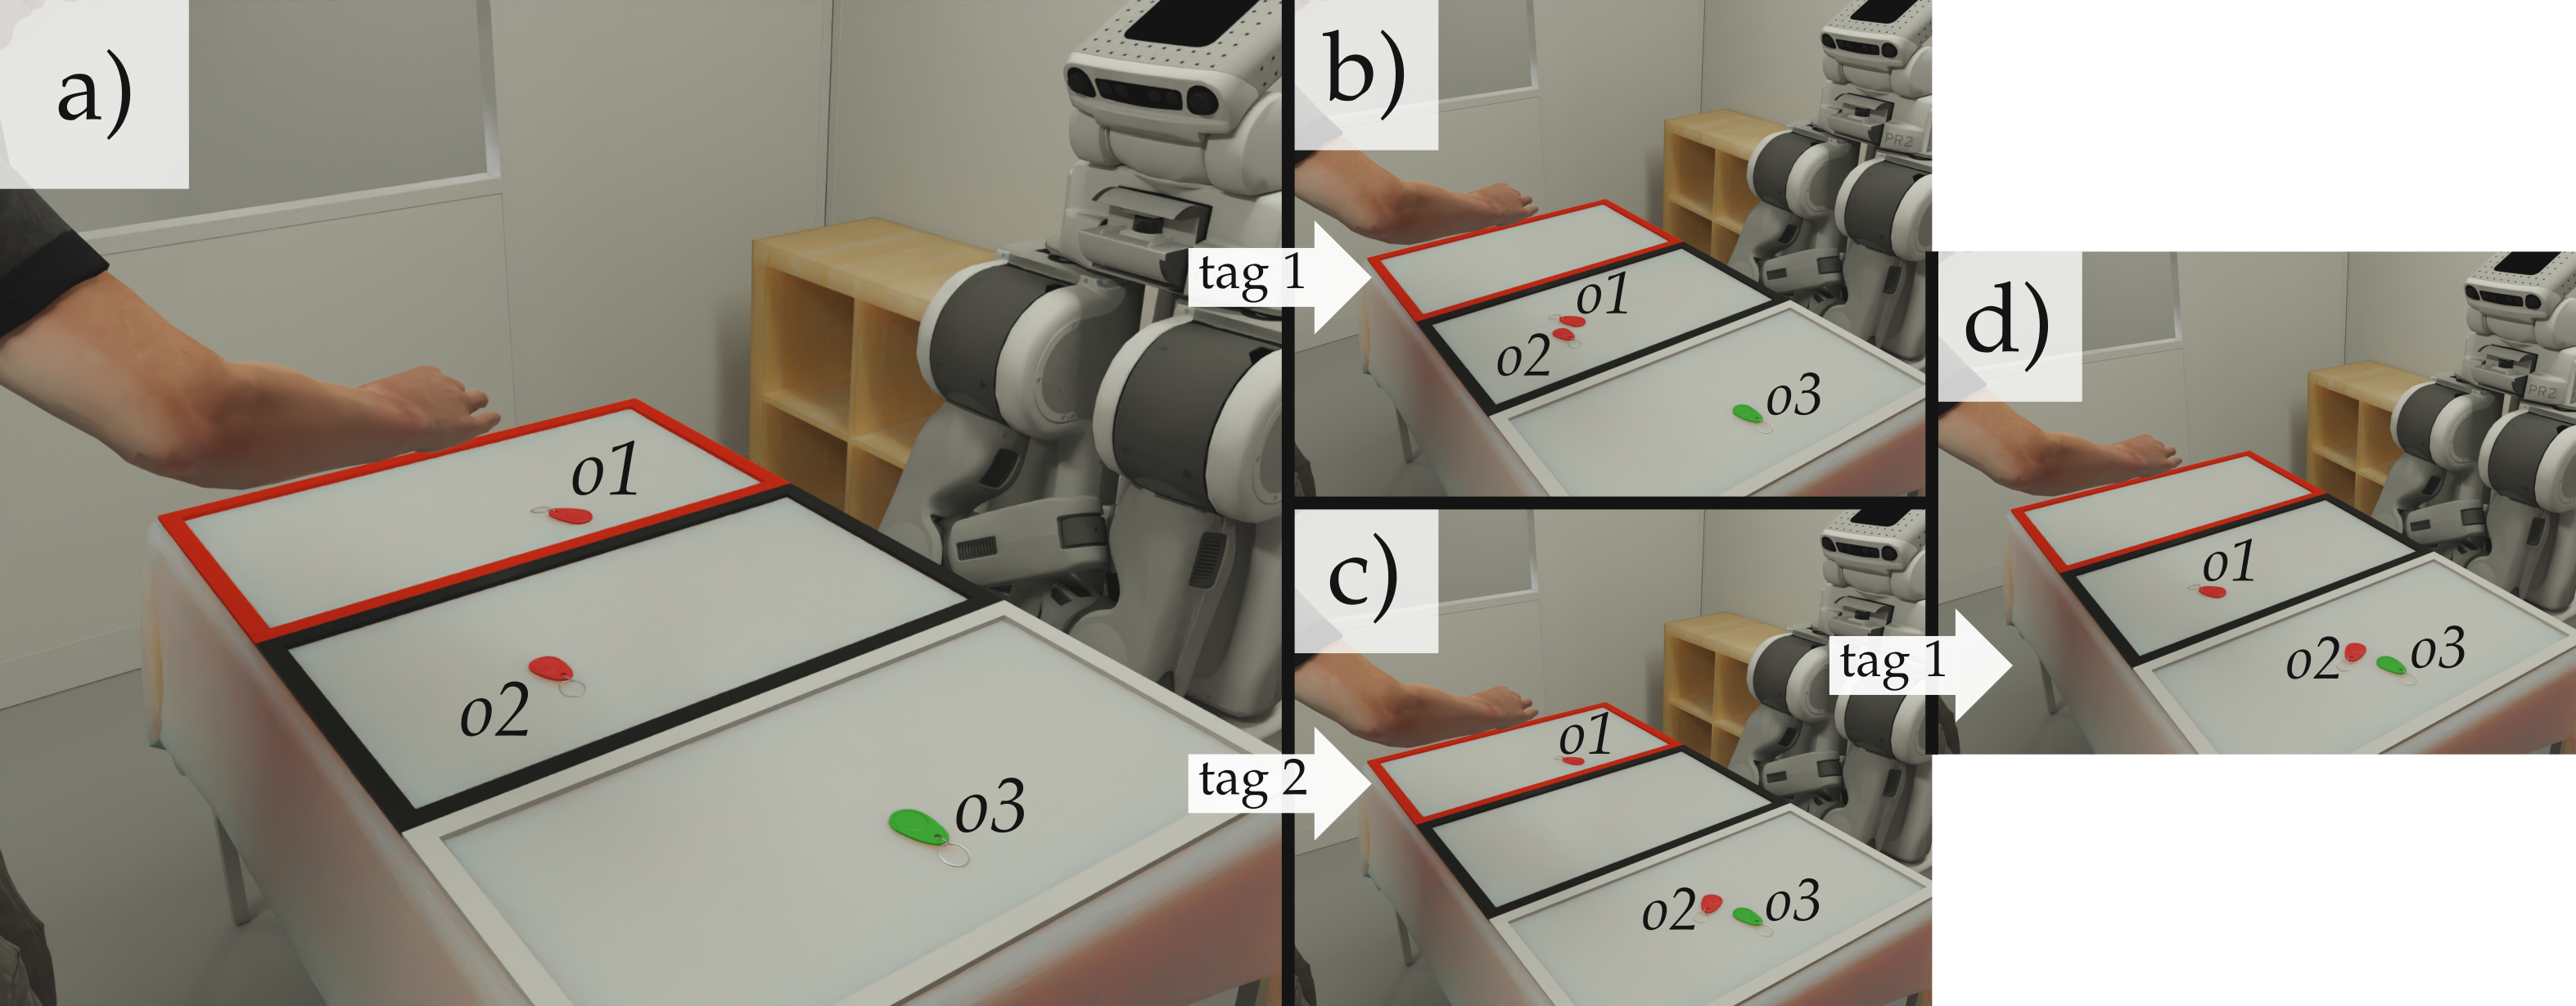
\includegraphics[width=\textwidth]{figures/chapter6/intro/intro.png}
\caption{\label{fig:chap6_intro} Referring to knife \textit{k2} in the current situation (\textit{t3}) is impossible if the robot is performing an action that does not allow it to see what is in front of the human. Considering a previous steps of the human's task, the robot can refer to the knife through the action to cut a tomato (\textit{t2}) or to cut a cucumber (\textit{t1}).}
\end{figure}

Consider the caption of the of an interaction represented in Figure~\ref{fig:chap6_intro} at the current instant \textit{t3}. The robot, in the back of the kitchen, has to ask the human for the knife \textit{k2}. Since the robot is performing another action of the joint task, it cannot see what is in front of the human. Consequently, it can know and thus use any spatial relations about \textit{k2}\footnote{We could also consider an object known by the robot but for which it does not have any information regarding its new location and searching for it. It would have to refer to it, to ask for the human help, without the possibility to use spatial relations.}. Therefore, the robot can only use \textit{k2} attributes (i.e. only it's color) to generate an expression referring to it. Still considering only the current instant \textit{t3}, two others blue knives hold in the kitchen being \textit{k1} and \textit{k3}. The knife \textit{k1} is attached to the wall in front of the robot meaning that it is already accessible to it and not to the human. This knife can thus be considered as being out of context and not leading to any ambiguity with \textit{k2}. The other blue knife \textit{k3} remains ambiguous since it does not have any perceptible attribute that differs from the one the robot has to refer to.

Until now, we only have considered the current situation \textit{t3} and not the human-robot shared experience about the task they perform. In the previous instant \textit{t2} the human was cutting a tomato with the knife \textit{k2}. At this previous instant, it was manifest to the human that the robot was observing the scene while he acted. This new information about the performed action could thus be used by the robot to generate a reference to the wanted knife in the current situation. A possible \acrshort{re} would be ``\textit{the knife with which you cut the tomato}''. 

Consider now the action a step before cutting the tomato at instant \textit{t1}. The human was cutting a cucumber with this same knife. The combination of these two past actions can be seen as the task of preparing vegetables. The robot can thus also use this knowledge to refer to the knife. A possible \acrshort{re} considering the totality of the interaction would be ``\textit{the knife with which you prepared the vegetables}''. The exploitation of shared knowledge about past activity in addition to the usual attributes and properties could lead to the generation of richer \acrshort{re} that could be easier to understand by the human partner. Besides, it allows extending REs use to contexts where the previous method was not effective.

This chapter is an extension of our previous work~\cite{buisan_2020_efficient} presented in chapter~\ref{chap:4}. It has been integrated within a cost-based Hierarchical agent-Base Task Planner to estimate the feasibility and cost of REs during the planning process~\cite{buisan_2020_human}, presented in chapter~\ref{chap:5}. In this chapter we will thus aim to create the inverse link, making the \acrshort{reg} able to use execution traces resulting from the execution of hierarchical plans generated by \acrshort{hatp}. Like the previous chapters, we only focus on the content determination of the \acrshort{reg} problem but continue to consider the need to have names in natural language to enable linguistic realization.

The main contribution of this chapter is an extension of the ontology-based \acrshort{reg} algorithm by \textbf{considering past agents' activities}. A side contribution of this chapter is a proposal of a formalism to \textbf{represent Hierarchical Execution Traces} (executed \acrshort{htn}-based plans) in an ontology. Our previous contribution considered cost functions based on the properties of the used relations to represent the cognitive load required for a human to interpret the \acrshort{re}. In this extension, we propose to add customizable cost functions based on time, to represent the cognitive load required for a human to remember referred activities.

First, we review the literature concerning \acrshort{htn} representation in ontologies and discuss \acrshort{reg}-related works that not only consider caption of situations. Then, we describe the used knowledge bases and the usual structure of \acrshort{htn} and shared \acrfull{het}. We then give in a first time an overview of how the knowledge bases should be updated and in a second time, the content of these updates in terms of how a shared \acrfull{het} is represented in an ontology. The extension of the algorithm is then detailed before ending with an efficiency comparison regarding the original version and a discussion around five illustrative cases to show the solutions found by our algorithm depending on the agent's knowledge about past activities.

\section{Related work}

In the previous chapter about Referring Expression Generation we already gave a good overview of the literature of the field. In this chapter, we thus briefly discuss few works trying to consider an interaction. We then move on to a wider part about the representation of \acrshort{htn} and execution traces in ontology to see the kind of information our algorithm could we to generate a new kind of referring expressions.

\subsection{Interaction based Referring expression}

\improvement{------more refs}
In all the previously presented works, the \acrshort{reg} is only performed on the current environment state. Williams in~\cite{williams_2020_toward} is the first to add a temporal aspect by considering a sequence of \acrshort{reg}. Like others before, he starts from the idea that to designate an entity it is preferable to use properties known by the hearer and that the latter will easily identify. Where others works, our included, represent that with cost on properties that we assume to be representative for the hearer, Williams tries to take advantage of an entire interaction. During such interaction, two partners will generate \acrshort{re}. The presented algorithm thus try to re-use properties used in previous descriptions made by the partner. In addition, he has implemented a forgetting model based on decay or interfering to avoid the use of properties used too long ago. This method has been tested on a ``Guess Who''-style game. This kind of game has the advantage that the used properties hold between the \acrshort{reg} and thus can be re-used. However, this assumption can no longer be maintained in a real dynamic interaction where objects are manipulated and their properties modified all along with the interaction.

Early in the field, Oberlander and Dale already showed that generating references to eventualities (\textit{i.e.} to past activities or past events) can be done in the same way as generating references to physical entities~\cite{oberlander_1991_generating}. However, they never generate references to entities through the use of past actions. To close this short tour, Wiriyathammabhum et al. in~\cite{wiriyathammabhum_2019_referring} use \acrshort{re} involving past actions to identify a referred entity in videos but does not generate them.

%The determination of the properties' costs will not be discussed here but we can mention \cite{belke_tracking_2002} and \cite{koolen_learning_2012} which use learning techniques to estimate the users' preferences.

\subsection{HTN-based tasks representation in ontology}

In robotic and even more in \acrshort{hri}, storing semantic information about past activities is needed to generate training data~\cite{diab_2020_knowing} and learn from experience~\cite{petit_2016_reasoning}, or to speak about what happened~\cite{mealier_2017_narrative}. Some approaches represent the past actions using structured sets of SQL tables~\cite{mealier_2017_narrative}, but such a representation lacks semantic information both on the involved entities (e.g. a robotic agent is a specific type of agent) and on the actions (e.g. a cut action is part of a salad preparation task). Since ontologies are fully suitable to represent semantic information about entities and their relations, they have been used to represent task planning knowledge. In~\cite{sun_2019_rtpo}, a Robot Task Planning Ontology (RTPO) is proposed but the model does not consider the rich semantics involved by the hierarchical nature and intricacies of human-robot joint activities. For example, they represent the fact that the action ``ChargeAction'' is a ``ChargeTask'' while a more correct semantic would be that the ``ChargeTask'' is composed of a ``ChargeAction''.

To represent episodes, the EASE-CRC has put forward the concept of narratively-enabled episodic memories(NEEMs)~\cite{diab_2020_knowing}. It is a log of perception events and sensor data annotated to give comprehensive logs of tasks performed by a robot. The annotations are based on the terminology provided by the Socio-physical Model of Activities(SOMA)~\cite{bessler_2020_foundations}. It proposes a high-level description of what s an event or an object in addition to the notion of plan. However, a plan is just a succession of actions and this terminology thus not support the use of \acrshort{het} for the moment. A design pattern for the representation of such NEEMs in ontology has been proposed in~\cite{bernd_2020_modelling}. However, this pattern is too cumbersome for ontology developers and not practical to use in side-fields we the safety of data input is not mandatory for the moment.

\acrshort{htn} is a very popular way for representing, planning, and controlling autonomous agents' activities \cite{ghallab_2004_automated, ingrand_2017_deliberation}. It is a tree representing how to decompose abstract tasks into primitive tasks directly applicable by an agent \cite{erol_1994_htn}. They are widely used for robotic planning as they allow to efficiently find complex plans by choosing between different task decompositions depending on the world state. 
Unlike more classical state-space search-based planning algorithms like STRIPS~\cite{fikes_1971_strips}, \acrshort{htn} planning does not explore applicable actions until a goal is reached, but rather tries to fully decompose an abstract task into applicable primitive tasks. Moreover, \acrshort{htn} planning is often quicker as domains (\acrshort{htn} representations) are provided with expert knowledge through the hierarchical structure and task decomposition alternatives. 
In \acrshort{hri} scenarios, their usefulness is even more apparent. In \cite{lallement_2014_hatp}, an \acrshort{htn} is used to generate human-robot joint plans. Furthermore, the hierarchical structure can be used to negotiate or communicate high-level plans when details do not matter~\cite{milliez_2016_using}. As an example, for a robot equipped with a charge plug and solar panels, an \acrshort{htn} may represent the abstract task of ``ChargeTask'' as being decomposed into either ``GoToChargeStation'' primitive (or abstract) task or ``GoOutside'' task. An \acrshort{htn} planner would then explore these alternatives and generate the most appropriate plan depending on the current world state: here the current weather.

To the best of our knowledge, few works exist on the representation of an \acrshort{htn} and their \acrfull{het} in ontologies. Umbrico et al. in~\cite{umbrico_2020_ontology} describe the notion of complex tasks composed of simple tasks but does not go further in the representation. In \cite{freitas_2014_using} only the planning domain is represented. The major issue is that the ontology classes are used to describe the general \acrshort{htn} concepts (i.e. action, method) while the field concepts (e.g. the cut task in our example) are described using the ontology individuals. Hence, this representation does not allow to represent abstracts or primitives tasks instantiations. This distinction between the domain as a high-level knowledge and thus represented in the ontology classes and properties and the \acrshort{het} representation as an instantiation of a domain is important to us. It allows to both represent how a given task could be done and how it has been done during execution. Our work is closer to BOWL~\cite{ko_2011_business}, an \acrshort{htn} ontology for business process representation. Even if they have defined some specific relations for the Business-to-Business field, the general tasks, decomposition, and tasks links representation are interesting. However, BOWL only represents the \acrshort{htn} and not \acrshort{het}s, but does not preclude it.

\section{Structuring and gathering the knowledge}

In this section, we present first the main knowledge structures necessary to perform the extended \acrshort{reg} through shared knowledge about past Human-Robot collaborative activity. We continue with an overview of the robotic architecture allowing us to acquire this knowledge, to understand the knowledge to be acquired offline and those to be acquired during the interaction. We end this section with the proposed terminology to represent \acrshort{htn} and \acrshort{het}s in the ontology.

\subsection{The three used knowledge representation}

Three knowledge representations are used and can be grouped into two categories: the dynamic and static ones. The dynamic part is updated all along the course of action, it is defined as $\kb = \langle \kbs, \kbe \rangle$ with $\kbs$ the semantic part already presented and $\kbe$ the episodic part. The static knowledge base represents the planning domain as a \acrfull{htn}.

\subsubsection{The Hierarchical Task Network}

In the previous chapter, we saw that an \acrshort{htn} is a way of representing a task to be planned, meaning to be fully refined and instantiated. In the present section, we go deeper into the \acrshort{htn} and give a more formal definition based on~\cite{erol_1994_htn}.

An \acrshort{htn}, noted $\HTN$, is defined as a set of tasks $\tasknetwork$. A task $\task$ is represented by a task name associated with a list of typed arguments. Taking the \acrshort{htn} illustrated in Figure~\ref{fig:chap6_domain}, the task \textit{cut} has the arguments \textit{A, V, K}, which are respectively an agent, a vegetable, and a knife. The general term task can be refined into \textbf{primitive task} ($\task \in \primtaskset$ with $\primtaskset$ the set of primitive tasks) or \textbf{abstract task} ($\task \in \abstaskset$ with $\abstaskset$ the set of abstract). A task is said to be primitive if it does not need refinement meaning that it can directly be executed by the robot or by a higher-level component\footnote{Primitive tasks usually have preconditions and effects, we are not describing in this thesis as not used.}. An abstract task needs further decomposition and can not be executed by the robot. In Figure~\ref{fig:chap6_domain}, \textit{PrepareSalad()} is an abstract task while \textit{cut(A,V,K)} is a primitive task.

Then, we define the set of decompositions $\decomposet$. A decomposition is a pair $(\abstracttask, \tasknetwork) \in \decomposet$ where $\abstracttask \in \abstaskset$ is an abstract task and $\tasknetwork$ a set of tasks describing one way of decomposing $\abstracttask$. In Fig.~\ref{fig:chap6_domain}, the abstract task \textit{PrepareVegetable(A,K,V)} has two decompositions \textit{d8} and \textit{d9}. Moreover, among the tasks set of a decomposition, can be enrich with a precedence order in which the tasks have to be performed. For example, in Figure~\ref{fig:chap6_domain}, the tasks \textit{peel(A, V, K)} and \textit{peel(A, V, K)} are totally ordered under the decomposition \textit{d8}. 

\begin{figure}[h!]
\centering
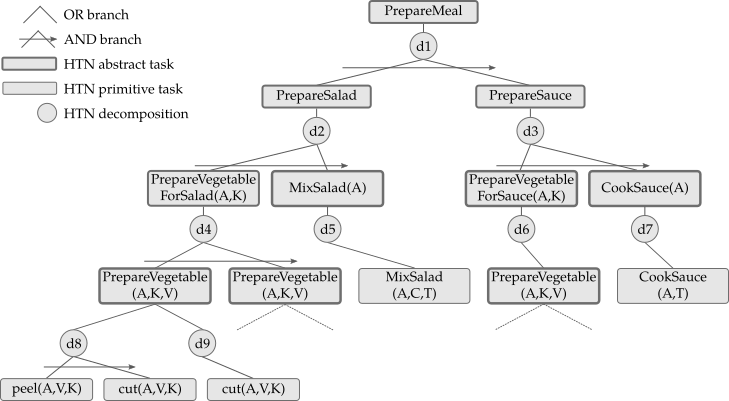
\includegraphics[width=\textwidth]{figures/chapter6/domain.png}
\caption{\label{fig:chap6_domain} The  domain of the high-level task \textit{PrepareMeal}. It is used by the planner (\acrshort{hatp}) to elaborate a Human-Robot shared plan through a context-based decomposition and parameter instantiation process (which vegetable V, which knife K, ...) including the selection of which agent A (Tony the human, or PR2 the robot) abstract tasks and/or primitive tasks will be allocated.}
\end{figure}

Given an initial world state and an initial task to decompose, a planner such as \acrshort{hatp} elaborates a plan through successive decompositions from the initial task and respecting the constraints issued by the initial world state. A resulting plan is a sequence of primitive tasks. The planner thus tries to recursively select a decomposition for each abstract task encountered until it reaches primitive tasks. Besides, the planner has to ground every argument of the tasks into entities of $\Abox$ (the ABox of the knowledge base $\kbs$) while respecting constraints regarding their types.

\subsubsection{The semantic and episodic knowledge bases}

The semantic knowledge base $\kbs$ is still an ontology as described earlier. The episodic knowledge base $\kbe$ is a timeline also called datebase~\cite{allen_1983_maintaining}. It maintains temporal reference for every fact that varies in time. Representing only the changes, we can assume that a fact holds between two changes.

We defined it as a pair $\kbe = ( \{ \langle \relation, \tau \rangle \}, \{ \langle \taction, \tinterval \rangle \} )$. The first element is a set of time-stamped relations like a classical datebase. The second element aims at representing the performed tasks. It is a set of pairs with $\taction$ an instance of a task and $\tinterval$ a temporal interval composed of two numerical values. The tasks defined in $\kbe$ are also represented as entities of $\kbs$ ($\taction \in \indivset$). Since they are semantically represented in $\kbs$ we can, inter alia, retrieve their types or arguments.

\begin{figure}[h!]
\centering
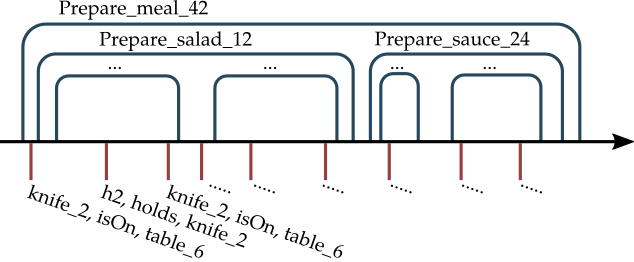
\includegraphics[scale=0.55]{figures/chapter6/ke.png}
\caption{\label{fig:chap6_ke} An example of timeline. In blue the performed tasks with their intervales and in red the relations changes.}
\end{figure}

Since we address \acrshort{hri} applications, in the same way, it has been done previously with the semantic knowledge base, we consider that the robot maintains a semantic and episodic knowledge base per human it is interacting with ($\kbs^{Hi}$ and $\kbe^{Hi}$ ) in addition to its own ($\kbs^{R}$ and $\kbe^{R}$). While the robot's own knowledge base is its personal truth, the agents' knowledge bases represent its estimation of the knowledge of its human partners.

\subsection{The knowledge gathering scheme}

We give now an overview of how the three knowledge bases are interconnected and how the semantic and episodic ones are updated. A minimal robotic architecture allowing the gathering of the necessary information is represented in Figure~\ref{fig:chap6_architecture}.

First of all, the task decomposition description stored as an \acrshort{htn} is parsed offline. We aim at extracting from it a semantic description of the tasks composing it (abstracts and primitives), their parameters, and their hierarchical links through the decompositions. All these descriptions are then stored into the ontology as classes and properties (dotted arrow on Fig.~\ref{fig:chap6_architecture}) in order to ground future executions traces.

Once the ontology initialized with a common ground of which the description of the planning domain is part, we can start the interaction. During the interaction, the situation assessment updates the semantic knowledge base of each agent with relations to the entities of the environment. Upon receipt of these facts, the semantic knowledge base temporally stamps them and stores them in the episodic knowledge base. Because it can also infer new facts thanks to the reasoning mechanisms, these inferred facts are also temporally stamped and stored in the episodic knowledge base\footnote{For now only the performed tasks will be used to generate the REs but we still wanted to have a more general scheme to understand the context in which we want to use it.}.

On request of the supervision module, the \acrshort{htn} planner takes its initial world state from the ontologies of the involved agents (1A) and generates a shared plan (1B). During the execution of the shared plan, the supervision describes the performed tasks semantically (detailed in the following subsection) (2A) and stamps them in the timeline (2B) with their respective begin and end times. While it knows the tasks performed by the robot, it needs to gather data from the episodic knowledge base of the human partner (2C), to monitor their tasks. The descriptions of the tasks are not stored in the episodic knowledge bases as not having any temporal mean. It would be nonsense to say that a task has a given parameter at a given time. We first describe it as having parameters on one side (2A) and then we describe when the task has been performed on the other side (2B). 

Upon a \acrshort{reg} request from the supervision, the \acrshort{reg} component explores the listener's both sematic and episodic knowledge bases (3) and returns the generated \acrshort{re} (4).

\begin{figure}[h!]
\centering
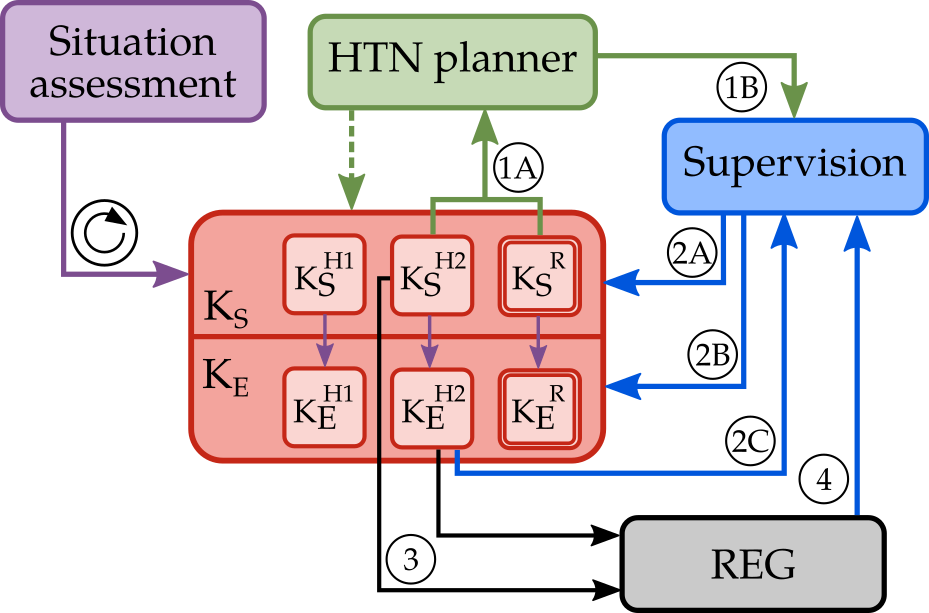
\includegraphics[scale=0.35]{figures/chapter6/architecture.png}
\caption{\label{fig:chap6_architecture} A ``minimal'' robotic architecture (on the base of the one of figure~\ref{fig:chap5_archi}) allowing to acquire and store the knowledge necessary to perform a \acrshort{reg} using the past human-robot activities. The dotted arrow represents an offline acquisition. The other arrows are online interactions between the components. The numbering represents the execution order during the execution of a task.
The robot knowledge bases ($\kbs^{R}$ and $\kbe^{R}$) and the estimated mental states of its human partners ($\kbs^{Hi}$ and $\kbe^{Hi}$) are updated permanently by the Situation Assessment component which tracks changes in the environment and by the robot supervisor which controls robot planning and execution activities and monitors humans actions.}
\end{figure}

When the supervision component inserts the executed tasks in the semantic knowledge base, it thus creates a \acrfull{het}. The execution trace can differ from the initial plan since it can be the result of plan repair or re-planning steps within the same global task achievement. The \acrshort{het} thus contains the actions which have been performed and their link to the higher level of abstraction. No forgetting mechanism is concidered since we focus on ``short'' interactions (few hours) but adding one would avoid the knowledge bases to grow indefinitely and also represent the human forgetting mechanism. This could be for future work.

\subsection{Building the ontology}

The aim of the following representation is not for planning per se (since this is done by the human-aware task planner) but rather to allow to store and manipulate a description of the execution of the human-robot shared plans together with their hierarchical structure and the information provided by the situation assessment component.
What is provided is the hierarchical task decomposition together with a semantic description of the entities used as tasks parameters, their properties, and relations to other entities in the environment. Moreover, the descriptions presented below are automatically generated from a \acrshort{hatp} domain and plan description~\cite{lallement_2014_hatp}.

\subsubsection{HTN in ontology}

An \acrshort{htn} represents the general knowledge about how to decompose high-level abstract tasks into executable primitive tasks. Since it is a piece of general knowledge, we represent it in the TBox and the RBox of the ontology. It allows instantiating the executed plan as individuals of the ontology.

\begin{figure}[h!]
\centering
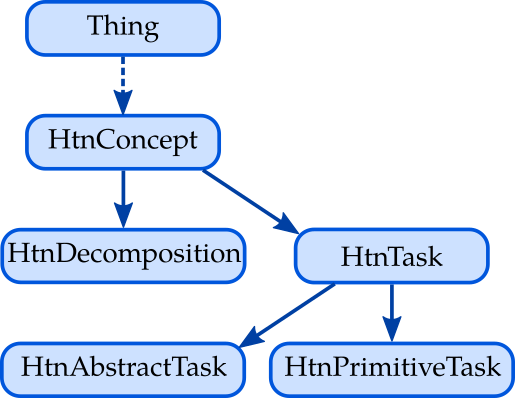
\includegraphics[scale=0.4]{figures/chapter6/tbox_base.png}
\caption{\label{fig:chap6_tbox_base} The upper classes used to decribe an \acrshort{htn}.}
\end{figure}

We first define the classes and properties common to any \acrshort{htn} representation.
As illustrated on Figure~\ref{fig:chap6_tbox_base}, the upper class in the TBox to describe an \acrshort{htn} is \textbf{HtnConcept} from which inherit the classes \textbf{HtnDecomposition} and \textbf{HtnTask}. The HtnTask class is then refined into \textbf{HtnAbstractTask} and \textbf{HtnPrimitiveTask}.
The RBox is composed without hierarchy of the properties \textbf{hasDecomposition}, \textbf{hasSubtask}, \textbf{hasParameter}, and their inverse (e.g. $(hasParameter, isParameterOf) \in \invset$). The property $hasDecomposition$ links an abstract task to its decompositions. The property $hasSubtask$ links a decomposition to the tasks (primitive or abstract) composing it. The property $hasParameter$ links a task to any other entity.

To represent an \acrshort{htn} $\HTN$ we thus create in the ontology a new class $\class$ for each :
\begin{enumerate}
	\item primitive task $\task$ such as 
$\task \in \primtaskset \Leftrightarrow \class \in \classset \wedge (\class,\ HtnPrimitiveTask) \in H$.
	\item abstract task $\abstracttask$ such as $\abstracttask \in \abstaskset \Leftrightarrow \class \in \classset \wedge (\class,\ HtnAbstractTask) \in H$.
	\item decomposition $\decompo$ such as $\decompo \in \decomposet \Leftrightarrow \class \in \classset \wedge (\class,\ HtnDecomposition) \in H$.
\end{enumerate}

For each decomposition $\decompo$ we describe the following relations using annotation properties:
\begin{enumerate}
	\item A decomposition come from an abstract task such as $\abstracttask \in \tasknetwork \Leftrightarrow (\abstracttask,\ hasDecomposition,\ \decompo) \in \annotationset$
	\item A decompositions has sub-tasks such as $\decompo \in \decomposet \Leftrightarrow (\decompo,\ hasSubtask,\ \task) \in \annotationset$.
\end{enumerate}

To put it into practice , let us consider the abstract task \textit{PrepareVegetable} of the domain illustrated in Figure~\ref{fig:chap6_domain}. The generated OWL representation of the listing~\ref{lst:chap6_owl_domain} is first composed of the \textit{PrepareVegetable} class inheriting from the \textit{HtnAbstractTask} concept. Through the use of the property \textit{hasDecomposition}, we state that the task has two decompositions being \textit{PVDecomp\_A} and \textit{PVDecomp\_B}. To refine these decomposition, we than create the \textit{PrepareVegetableDecomp} class inheriting from the \textit{HtnDecomposition} concept. It will be use to group all the decomposition of the \textit{PrepareVegetable} abstract task. Considering the fisrt decomposition (\textit{d8} on Figure~\ref{fig:chap6_domain}), we create a new class for it. The class \textit{PVDecomp\_A} thus inherite of \textit{PrepareVegetableDecomp}. This decomposition is composed of two sub-tasks \textit{Cut} and \textit{Peel}.  However, to keep track of the fact that thay have to be executed in the context of the said decomposition we refine them. We define \textit{Cut\_PVDecomp\_A} and \textit{Peel\_PVDecomp\_A} respectively inheriting of the primitives tasks \textit{Cut} and \textit{Peel}. With the property \textit{hasSubtask} we then describe that \textit{PVDecomp\_A} has two sub-tasks \textit{Cut\_PVDecomp\_A} and \textit{Peel\_PVDecomp\_A}.

Even if a task is used several times in the same \acrshort{htn}, it will be described only once.

\begin{lstlisting}[frame=single, basicstyle=\scriptsize\ttfamily, label={lst:chap6_owl_domain}, caption={Description of the abstract task PrepareVegetable and one of its decomposition in the OWL language using the Turle syntax.},captionpos=b, style=OwlTurtle]
:PrepareVegetable rdf:type owl:Class ;
                  rdfs:subClassOf :HtnAbstractTask ;
                  :hasDecomposition :PVDecomp_A ;
                  :hasDecomposition :PVDecomp_B .

:PrepareVegetableDecomp rdf:type owl:Class ;
                        rdfs:subClassOf :HtnDecomposition .

:PVDecomp_A rdf:type owl:Class ;
            rdfs:subClassOf :PrepareVegetableDecomp ;
            :hasSubtask :Cut_PvDecomp_A ;
            :hasSubtask :Peel_PvDecomp_A .

:Cut_PvDecomp_A rdf:type owl:Class ;
                rdfs:subClassOf :Cut .
\end{lstlisting}

In the latter description we have only represented the hierarchy of the tasks. We now need to specify the parameters of each task. They are represented using the upper property \textit{hasParameter}. At the difference to se ones used to describe the hierarchy, these aim to be used to instantiate executed tasks. Indeed, this property is first refined into several ones, being \textit{hasParameter.i} with $i \in \mathbb{N}$. This refinement level describes the position of each parameter in the tasks arguments list. We thus have hasParameter.0 the property for the first parameter of an argument list, hasParameter.1 the property for the second one, etc. These refinements are independent of the translated \acrshort{htn}.

\begin{figure}[h!]
\centering
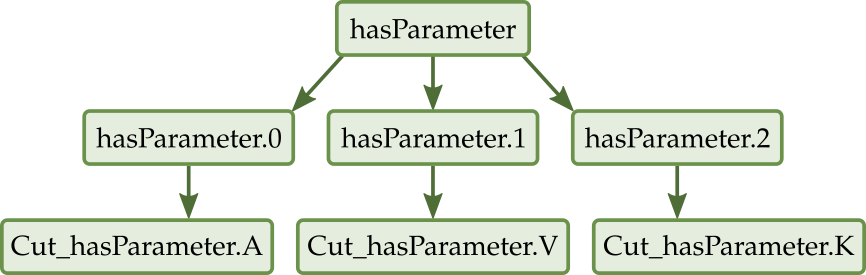
\includegraphics[scale=0.4]{figures/chapter6/rbox_params.png}
\caption{\label{fig:chap6_rbox_params} The properties hierarchy for the parameters of the \textit{Cut} task.}
\end{figure}

Each of these properties is then refined and specified for every task of the \acrshort{htn} to describe. This second specification aims at representing the parameters with their name in the task parameters list, their position isn the parameter list, and the type of entities they can be bounded to. Taking the example of the primitive task \textit{Cut} of Figure~\ref{fig:chap6_domain}, the generated description is presented in listing~\ref{lst:chap6_owl_params}. The parameter \textit{A} of the \textit{Cut} task is at position 0 of the parameter list. We thus define the property \textit{Cut\_hasParameter.A} as a refinement of the property \textit{hasParameter.0}. The resulting hierarchy is illustrated on Figure~\ref{fig:chap6_rbox_params} pour the parameters of the \textit{Cut} task. The parameter \textit{Cut\_hasParameter.A} aims at representing the agent performing the task. Consequently, the property has to link an \textit{Cut} task to an agent. We represent it respectively with the domain and the range of the property. The same process is performed for every parameter of each task.

\begin{lstlisting}[frame=single, basicstyle=\scriptsize\ttfamily, label={lst:chap6_owl_params}, caption={Description of the \textit{hasParameter} property specifications for the parameters (resp. the agent performing the task, the cut vegetable, and the used knife) of the \textit{Cut} primitive task in the OWL language using the Turle syntax.},captionpos=b, style=OwlTurtle]
:Cut_hasParameter.A rdf:type owl:ObjectProperty ;
                    rdfs:subPropertyOf :hasParameter.0 ;
                    rdfs:domain :Cut ;
                    rdfs:range :Agent .

:Cut_hasParameter.V rdf:type owl:ObjectProperty ;
                    rdfs:subPropertyOf :hasParameter.1 ;
                    rdfs:domain :Cut ;
                    rdfs:range :Vegetable .

:Cut_hasParameter.K rdf:type owl:ObjectProperty ;
                    rdfs:subPropertyOf :hasParameter.2 ;
                    rdfs:domain :Cut ;
                    rdfs:range :Knife .
\end{lstlisting}

\subsubsection{HET in ontology}

As explained with the gathering scheme, the \acrshort{htn} planner (here \acrshort{hatp}) generates a hierarchical plan for a given human-robot collaborative task that is then executed by the robot and its human partner. Whenever a task (abstract or primitive) is executed by the robot or its execution by the human is perceived, its description is inserted in the agents' KBs. These executed tasks are thus instances of tasks and have to be grounded to the \acrshort{htn} described in the ontology.

\begin{lstlisting}[frame=single, basicstyle=\scriptsize\ttfamily, label={lst:chap6_owl_plan}, caption={A partial description of the initiation of a decomposition of a PrepareVegetable task and its primitive Cut task resulting from a plan and linked to the description of the domain. Description is provided in the OWL language using the Turle syntax.},captionpos=b, style=OwlTurtle_indiv]
:pv_3 rdf:type owl:NamedIndividual ;
      rdf:type :PrepareVegetable ;
      :hasDecomposition :decomp_pv_3 .

:decomp_pv_3 rdf:type owl:NamedIndividual ;
             rdf:type :PVDecomp_A ;
             :hasSubtask :peel_5 ;
             :hasSubtask :cut_7 .

:cut_7 rdf:type owl:NamedIndividual ;
       rdf:type :Cut_PVDecomp_A ;
       :Cut_hasParameter.A :tony ;
       :Cut_hasParameter.V :c1 ;
       :Cut_hasParameter.K :k2 ;
\end{lstlisting}

To explain how the task instances are described in the ontology, let us take the example of an agent executing a decomposition of the abstract task \textit{PrepareVegetable}. A partial representation of this instance is represented in the listing~\ref{lst:chap6_owl_plan} and drawn on Figure~\ref{fig:chap6_abox}.

The human partner has performed \textit{decomp\_pv\_3}, an instance of the decomposition \textit{PVDecomp\_A} being the first decomposition of the abstract task \textit{pv\_3} that is a \textit{PrepareVegetable} abstract task. \textit{pv\_3} is thus an insatnce of the class \textit{PrepareVegetable} and \textit{decomp\_pv\_3} and instance of the class \textit{PVDecomp\_A}. We use the property \textit{hasDecomposition} to state that \textit{pv\_3} has been acheived with the decomposition \textit{decomp\_pv\_3}. Then, with the property \textit{hasSubtask}, we describe that \textit{decomp\_pv\_3} is composed of two instantiated sub-tasks \textit{peel\_5} and \textit{cut\_7}.

The primitive task \textit{cut\_7} is a \textit{Cut} task but has been acheived in the context of the first edcomposition of the abstract task \textit{pv\_3}. The individual \textit{cut\_7} thus inherite of the class  \textit{Cut\_PVDecomp\_A}. Because the \textit{Cut} task has three parameters, they have to be instantiated. To do so, we use the made refinements of the property \textit{hasParameter}. Here the task has been performed by the human \textit{tony} how has cut the cucumber \textit{c1} with the knife \textit{k2}. The instance \textit{cut\_7} is linked with \textit{tony} through the property \textit{Cut\_hasParameter.A}, with \textit{c1} the property \textit{Cut\_hasParameter.V}, and with \textit{k2} the property \textit{Cut\_hasParameter.K}. All these instances conrespond to the range of each property being respectively an agent, a vegetable, and a knife. The same process should be done for the primitive task \textit{peel\_5}. Moreover, the abstract task \textit{PrepareVegetable} having also three parameters, we should also link \textit{pv\_3} with its instantiated parameters.

\begin{figure}[h!]
\centering
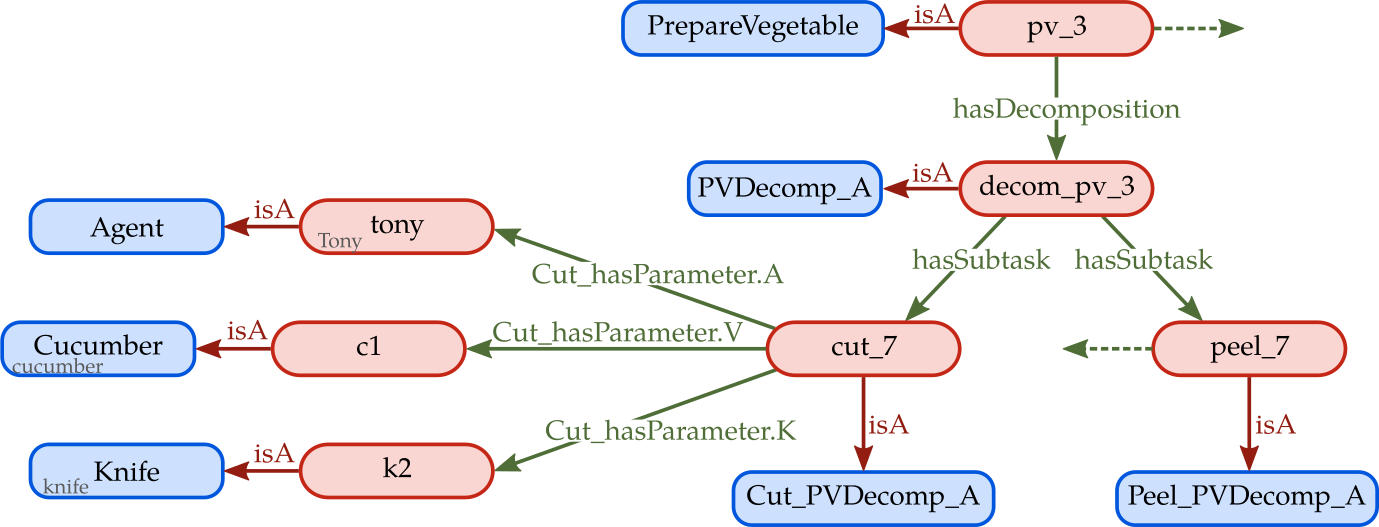
\includegraphics[width=\textwidth]{figures/chapter6/abox.png}
\caption{\label{fig:chap6_abox} A graphical representation of the instance of a decomposition of the abstract task \textit{PrepareVegetable}.}
\end{figure}

\section[REG algorithm modifications]{Modifying the REG algorithm to support the past experiences}

Now the Hierarchical Execution Traces are described in the ontology, we present in this section how we have modified the original \acrfull{ucs} \acrshort{reg} algorithm to make it able to use this new knowledge.

The first assumption we made to use tasks in a \acrshort{reg} solution is that for each task involved in the solution, all its parameters must be part of the solution. This constraint to get all the parameters of a task is important for linguistic realization. If this constraint were not satisfied, we could have results where even the agent having performed the task would not be referred\footnote{This constraint could be an important limitation. It will be discussed in an exploratory work in the next chapter.}.

\begin{theorem} [The complete instantiation]
\label{the:complete_intance}
For any task $\task$ appearing in a \acrshort{re}, all its parameters $\property \in \propset | (\property,\ hasParameter) \in \inclset \wedge (\property, \task) \in \domainset$ must exist in the solution.
\end{theorem}

The $\goaltest$ function which assesses if a node is a goal is modified according to this constraint. In addition to test if $\mathcal{M}(\var_t) = \goalindiv$, it checks if every past tasks used in $\mathcal{T}$ are assigned with all their parameters.

Now we can test if a goal node involves all the parameters of a task, we expand the function finding new actions for the \acrshort{ucs} algorithm. To not confuse the reader between the actions of the \acrshort{ucs} and the actions that a robot can perform, we will rather use the term ``addition'' to speak about relations that can be added to a candidate \acrshort{re} in order to find a solution. We thus adapt the $\additions$ function to explore past tasks and their parameters (Alg.~\ref{alg:chap6_additions}).

\begin{algorithm}[htb!]
\caption{\label{alg:chap6_additions} The modified $\additions$ function with the two newly introduced sub-functions}

\begin{algorithmic}

    \Function{\additions}{$node$} 
        \State $sucess, additions\leftarrow$ \typingadditions($node$)
        \If{$sucess = True\ and\ additions \neq \emptyset$}
            \Return $additions$
        \EndIf
        
        \State $additions\leftarrow$ \completionadditions($node$) \Comment{new introduced function}
        
        \If{$additions \neq \emptyset$}
            \Return $additions$
        \EndIf
        
        \State $additions\leftarrow$ \actingadditions($node$) \Comment{new introduced function}
        \State $additions\leftarrow additions\ \cup$ \differenceadditions($node$) 
        
        \Return $additions$
    \EndFunction
    
\end{algorithmic}
\end{algorithm}

While the $\differenceadditions$ aims at exploring relations that differ from other ambiguous entities, the $\actingadditions$ complements it by exploring the tasks in which the ambiguous entities involved in the candidate \acrshort{re} are part of. In the latter, for each variable $\var_i$ of $\mathcal{M}$ having several substitutions, we search in $\kbs$ all relations involving the anonymous entity $\indiv_i$ and an abtract or primitive task. This means tha we are looking all the relations $\relation = (\indiv_i,\ \property,\ \indiv_{task}) \in \relationset\ |\ (\property,\ isParameterOf) \in \inclset \wedge (\indiv_{task}, HtnTask) \in \inheritset$.

The second added function, $\completionadditions$, aims at making the \acrshort{re} valid. It ensures that any task used in a candidate \acrshort{re} has all its parameter inserted in that \acrshort{re}. For every task $\indiv_{task}$ used in a relation of $\mathcal{T}$ we search in $\relationset$ all the relations of having for subject $\indiv_{task}$ and for predicate a property inheriting from $hasParameter$. Among all these relations, we add to the possible additions of the current node the once not present in $\mathcal{T}$.

Regarding the order in which the functions of additions are performed, we always start with the ones aiming to make the candidate \acrshort{re} valid. First, we try to type any anonymous entity. If typing additions have been found or some should have been found but were not, the function stop here. In the case where some have been found we thus type the anonymous entities. In the other case, not additions will be generated and the explored branch will be disused. If every anonymous entity is already typed, we try to complete the tasks involved in the candidate \acrshort{re}. If additions have to be done, we stop here and return them. By the way, this means that the next evaluation of this candidate \acrshort{re}, the newly introduced entity will be typed first before continuing to complete the involved tasks. If every involved task has all their parameter, then and only then, we try to find new actions based on differences or on past tasks.

The cost of an addition representing a task (i.e. an addition involving the property $hasParameter$ or $isParameterOf$) is the cost of the task itself divided by the number of parameters. We chose to process in this way to avoid zero-cost addition and because every inserted parameter will already have a cost due to at least their typing. Thanks to the episodic \acrshort{kb}, the cost of these additions can also be weighted depending on the amount of time passed since the task has been performed. This meets the decay theory used in \cite{williams_2020_toward} and makes a preference over the more recent which could be easier to remember for the \acrshort{re} receiver. The determination of the properties' costs and tasks' costs will not be discussed here but we can mention \cite{belke_2002_tracking} and \cite{koolen_2012_learning} which use learning techniques to estimate them.

Using the presented algorithm, a reference solution to refer to a knife through the primitive task \textit{peel(A,V,K)} of the \acrshort{htn} of Figure~\ref{fig:chap6_domain} could be : \textit{(?0 isA Knife), (?0 isParameterOf ?1), (?1 isA peel), (?1 hasParameter Tony), (?1 hasParameter ?2), (?2 isA Cucumber)}. The variable ?0 represents the referred knife and the variable ?1 represents the task to which the knife is associated. It could be verbalized as \textit{``The knife with which Tony peel the cucumber''}.

\section{Results}

We present hereafter the solutions found by our algorithm on an illustrative example and show how the tasks estimated to be known to the \acrshort{re} hearer can impact the algorithm solution. Then, we discuss execution time measures to analyze the impact of such an extension regarding the original version of the \acrshort{ucs}-\acrshort{reg} algorithm.

\subsection{One execution trace for five referring expressions}

Let us take activities of the introduction example (Figure~\ref{fig:chap6_intro}) related to the \acrshort{htn} of Figure~\ref{fig:chap6_domain}. With this \acrshort{htn}, a planner has elaborated a shared hierarchical plan illustrated in Figure~\ref{fig:chap6_meal_plan}. The primitive tasks are listed and organized according to a timeline. The abstract tasks hierarchy is shown on the right. The planner has assigned the tasks to two agents; a robot (pr2) and a human (tony).

We introduce a third agent, the human Bob. He is a spectator of the shared activity. We define five cases depending on the moments when Bob is in the kitchen where Pr2 and Tony are collaborating for the meal preparation. The colored lines, next to the timeline, represent the moments where Bob is in the kitchen for each case. For example, in case 1 (black line), Bob is only aware of the tasks primitive tasks \textit{Cut(tony,t2,k1)} and \textit{CookSauce(Pr2, t2)}. The primitive tasks the robot estimated Bob to be aware of are thus added to his knowledge bases, both semantic and episodic. Moreover, if an agent is aware of all the tasks (primitive or abstract) composing an abstract task, he is also aware of the abstract task. In the first case, Bob is thus aware of the abstract tasks \textit{PrepareVegetable(tony, t2, k1)},\textit{PrepareVegetableForSauce(tony, k1)}, \textit{CookSauce(pr2)}, and \textit{PrepareSauce()}.

\begin{figure}[ht!]
\centering
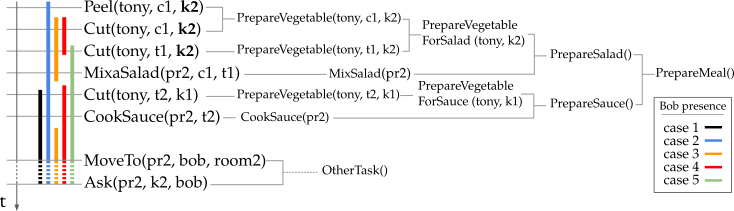
\includegraphics[width=\textwidth]{figures/chapter6/prepare_meal_plan.png}
\caption{\label{fig:chap6_meal_plan} The hierarchical execution trace to prepare the meal and a trace for another subsequent high-level task, organized according to a timeline. In the current instant, PR2 is asking Bob, a second human, for knife \textit{k2}. The five cases are represented by five colors at the left of the tasks and correspond to tasks seen by Bob, the human spectator. In case 1, Bob did not see any tasks involved in the preparation of the salad but was present during the sauce preparation. In the second case, he observed all the activities.}
\end{figure}

In all five cases, the goal is for Pr2 to refer to the knife \textit{k2} to Bob. We assume that the communication about it occurs out of the kitchen. This means that no spatial knowledge is available to generate the \acrshort{re}. We present hereafter the solutions found for each of the cases and detail how they have been found.

\paragraph{Case 1:} The algorithm first types \textit{k2} as being a Knife with the function $\typingadditions$.
Since no task is involved for now in the candidate \acrshort{re}, the $\completionadditions$ does not find any additions. Then, because Bob is not aware of any past task involving \textit{k2}, the $\actingadditions$ does not find addition either. Other relations, such as its color, can be added by the $\differenceadditions$ but none allow to solve the ambiguity. As a result, no solution can be found in this case.

\paragraph{Case 2:} The $\typingadditions$ function first type \textit{k2}. Then, the $\completionadditions$ function has nothing to complete. This time all the tasks (primitive and abstract) performed by Pr2 and Tony are known by Bob. Among them, three primitive tasks and three abstract tasks involve \textit{k2}. The $\actingadditions$ function thus propose six additions of the form $(k2,\ isParameterOf,\ \indiv_t)$ with $\indiv_t$ being the instances of the tasks. The $\differenceadditions$ function has only one possible addition being the color of $k2$. However, it does not help to solve the ambiguity and will give the same solutions as the other candidate \acrshort{re}, with one more relation making it more costly than the others at each step. In the five new nodes to explore involving tasks, the tasks are not labelled and are thus typed. At the next loop, because every candidate \acrshort{re} under exploration involves a task, the $\completionadditions$ function adds one new parameter for each using relation with the $hasParameter$ property. Considering the addition of the agent having performed the tasks, they both have a label and do not need to be typed. Because the abstract task \textit{PrepareVegetableForSalad} has only two parameters while the five others have three parameters, the node exploring it is found to be valid at this step while the others are not. The parameter of the knife has been added by the relation $(k2,\ isParameterOf,\ \indiv_t)$ and the parameter of the agent has been added by the relation $(\indiv_t,\ hasParameter,\ tony)$. The solution \acrshort{re} is: \textit{(?0 isA Knife), (?0 isParameterOf ?1), (?1 isA PrepareVegetableForSalad), (?1 hasParameter tony)}. Matching it in the knowledge base gives only one substitution for the variable ?0 being the target entity \textit{k2}. The verbalization\footnote{The proposed verbalization is automatically generated as proof of usability but the algorithm is not presented here.} would be \textit{``the knife with which Tony prepared the salad vegetables''}.

\paragraph{Case 3:} In this situation, Bob is only aware of two primitive tasks involving \textit{k2} being cutting tasks and one abstract task being a \textit{PrepareVegetable}. Because all have three parameters, at the difference of the previous case, the third parameter of each task is also explored and typed in a second time. At this step, all active nodes are valid. Because all have the same number of parameters, their cost difference depends on the time. The node with the lowest cost is the one with the more recent task. It could either be the second cut task of the abstract task of the vegetable preparation. We could prefer the most precise one being the cut task. The solution \acrshort{re} is: \textit{(?0 isA Knife), (?0 isParameterOf ?1), (?1 isA Cut), (?1 hasParameter tony), (?1 hasParameter ?2), (?2 isA tomato)}. Only one substitution exists for the variable ?0 being the target entity. The verbalization would be \textit{``the knife with which Tony cut the tomato''}.

\paragraph{Case 4:} Previously, even if Tony had cut another tomato with another knife, it did not lead to any ambiguity since it was estimated as unknown by Bob. This time, Bob knows that Tony cut two different tomatoes with two knives so the previous solution is not a goal node anymore since two substitutions exist for the variable ?0. The algorithm thus refers to the knife through the cut task on the cucumber \textit{c1}. The verbalization would be \textit{``the knife with which Tony cut the cucumber''}.

\paragraph{Case 5:} In this last case, the only task involving the knife \textit{k2} estimated to be known by Bob is Alex cutting the tomato \textit{t1}. However, Bob knew another cutting task with the tomato \textit{t2} but with the knife \textit{k1} which leads to ambiguity. The algorithm chose anyway the cut task as it is the only possibility. Despite this, our algorithm is able to find a solution by specifying the diverging argument that is the tomato. The tomato \textit{t1} being involved in the \textit{MixSalad} abstract task, the algorithm is able to use this second task to specify the argument of the first one. The solution \acrshort{re} is: \textit{(?0 isA Knife), (?0 isParameterOf ?1), (?1 isA Cut), (?1 hasParameter tony), (?1 hasParameter ?2), (?2 isA tomato), (?2 isParameterOf ?3), (?3 isA MixSalad), (?3 hasParameter pr2), (?3 hasParameter ?4), (?4 isA Cucumber)}. Matching it in the knowledge base gives only one substitution for the variable ?0 being the target entity \textit{k2}. The verbalization would be \textit{``the knife with which Tony cut the tomato that I mixed with the cucumber''}.

Over these five case study, we saw that the algorithm is able to use either primitive or abstract tasks, to consider the moment where the tasks have been performed to choose the most appropriate one, and to use several tasks in a single \acrshort{re}.

\subsection{The impact of the extention on the performances}

With the previous results, we saw the kind of solution the algorithm can generate. With this new test, we want to assess the impact of the proposed extension, in terms of execution time, regarding the original version. To do so, we have chosen the realistically-sized knowledge base (101 entities, 36 classes, 40 properties, and 497 relations) used to evaluate the original version. For recall, it describes an apartment with three rooms including several pieces of furniture (tables, shelves) and objects (cups, boxes) linked through spatial relations (isAtLeftOf, isOn) and attributes (hasColor, hasWeight). Both the original algorithm and its extended version have been run over all the 77 entities inheriting from the ``Object'' class, representing physical entities. The knowledge base is still managed using the Ontologenius system and we do not pass by the ROS services to not be impacted by the communication time in our measures.

On this ontology not having tasks described in it, the extension has a negligible impact. The average execution time is about 1.04ms for the original algorithm versus 1.16ms for the extension. Even for the most complex case, we pass from 6.25ms to 6.86ms. This difference can be due to the search of tasks even if none is present in the ontology.

To estimate the impact when tasks are present in the ontology, we chose to put ourselves in the worst case where tasks are described but can not be used to find a solution. To create this worst case, we add two actions, each having three parameters, to each object described in the apartment. Even if each action is unique (an individual per action), all are of the same type and have the same entities as parameters. In this way, the tasks will be explored but will lead to ambiguity, creating only an overload for the exented algorithm. Consequently, the solutions of both algorithms should be the same. The tasks description leads to an addition of 144 entities to the ontology (the 144 tasks) and 432 relations (three parameters per task). We estimated that such an amount of tasks could be the result of several hours of interaction. With this new setup, the impact of the extension is much more noticeable. For the most complex entity needing six relations in its solution, we pass from 6.40ms to 70.57ms. We note that 75\% of the entities are solved under 5.96ms versus 1.32, 50\% under 1.53ms versus 0.51ms, and 25\% under 0.50ms versus 0.19ms. In addition, we observe that the longer the \acrshort{re} is to compute with the original version, the more noticeable the impact of the extension is. Moreover, because the more relations is needed, the longer the \acrshort{re} is to compute, we find here a part of the explanation. For each node coming from a difference addition, two additions representing tasks are proposed at the next step. We thus add two to the original branching factor, having an exponential impact on the number of generated node and thus on the execution time. However, in an \acrshort{hri} context, even the worst case is still acceptable and will not spoil the interaction. Moreover, we have put ourselves in the worst case where the added tasks can not be used to generate the \acrshort{re}. In more realistic cases, we would have a diversity of tasks and their use in the \acrshort{reg} may allow us to reduce the solution length for the most complex cases and hence reduce the average execution time.

%chap 4
%count    77.000000
%mean      1.080750
%std       1.355236
%min       0.013237
%25%       0.193782
%50%       0.516371
%75%       1.322064
%max       6.405807

%count    77.000000
%mean      5.531283
%std       9.780631
%min       0.012952
%25%       0.509738
%50%       1.538461
%75%       5.968753
%max      70.577606

%2    27
%3    21
%4    14
%5     9
%1     5
%6     1

\section{Discussion}

The contribution presented in this section allows the generation of a new kind of Referring Expression but at the cost of a longer computational time and with the constraint of a precise task description. Moreover, due to the need to use all the parameters of a task, the \acrshort{htn} has to be designed with the goal to be used for \acrshort{reg}.

We can identify three major limitations of the current contribution:
\begin{itemize}
  \item Because we consider the linguistic realization without any consideration of the combination of parameter allowing the generation of a sentence, all the parameters have to be used.
  \item Because the additions consist of the addition of a single relation at the time, all the parameters can not be inserted in a single addition. The consequence is an increase of the branching factor and thus of the execution time.
  \item Because the algorithm search for relations with precise properties in it, the method can not be applied to any task description such as the SOMA~\cite{bessler_2020_foundations} one.
\end{itemize}

These limitations will be discussed in detail in the next chapter through a preliminary work aiming to generalize the Referring Expression Generation that supports the use of past shared task.